%%%%%%%%%%%%%%%%%%%%%%%%%%%%%%%%%%%%

\section{Considering categorical data}

%%%%%%%%%%%%%%%%%%%%%%%%%%%%%%%%%%%%

\subsection{Contingency tables and bar plots}

%%%%%%%%%%%%%%%%%%%%%%%%%%%%%%%%%%%%

\begin{frame}
\frametitle{Contingency tables}

A table that summarizes data for two categorical variables is called a \hl{contingency table}.

$\:$ \\
\pause
The contingency table below shows the distribution of students' genders and whether or not they are looking for a spouse while in college.

\begin{center}
\begin{tabular}{l l cc rr}
					& 			& \multicolumn{2}{c}{{looking for spouse}} \\
  \cline{3-4}
					&			& No	& Yes	& Total & \hspace{3mm}  \\ 
  \cline{2-5}
\multirow{2}{*}{{gender}}& Female 		& 86 	& 51 		& 137 \\ 
  					& Male 		& 52 	& 18	 	& 70\\ 
  \cline{2-5}
  					& Total		& 138& 69	&  207 \\
  \cline{2-5}
\end{tabular}
\end{center}

\end{frame}

%%%%%%%%%%%%%%%%%%%%%%%%%%%%%%%%%%%%

\begin{frame}
\frametitle{Bar plots}

A \hl{bar plot} is a common way to display a single categorical variable. A bar plot where proportions instead of frequencies are shown is called a \hl{relative frequency bar plot}.

\begin{center}
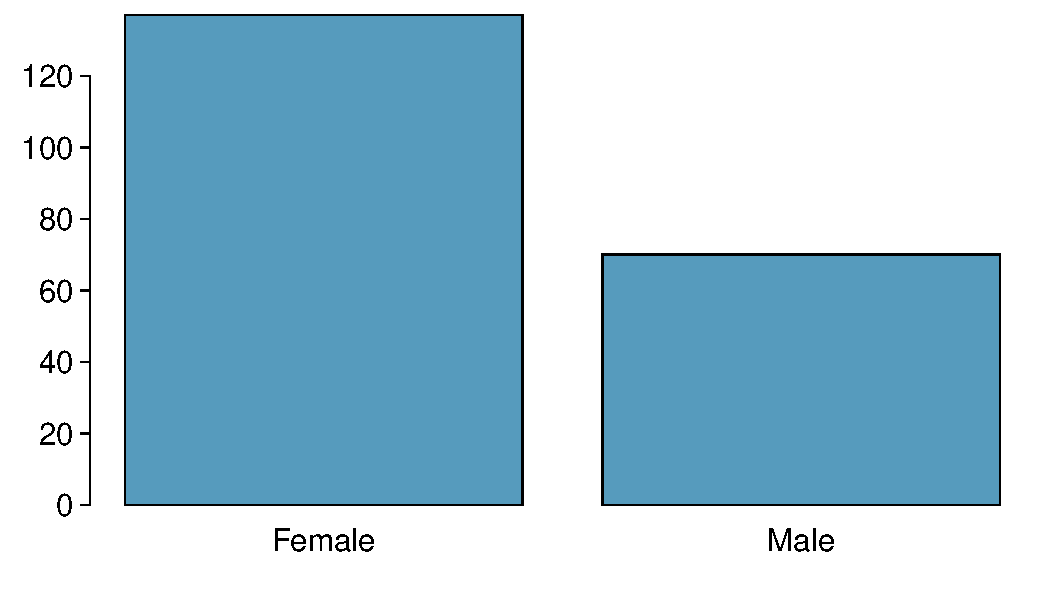
\includegraphics[width=0.4\textwidth]{1-7_categorical_data/figures/gender_spouse/gender_bar}
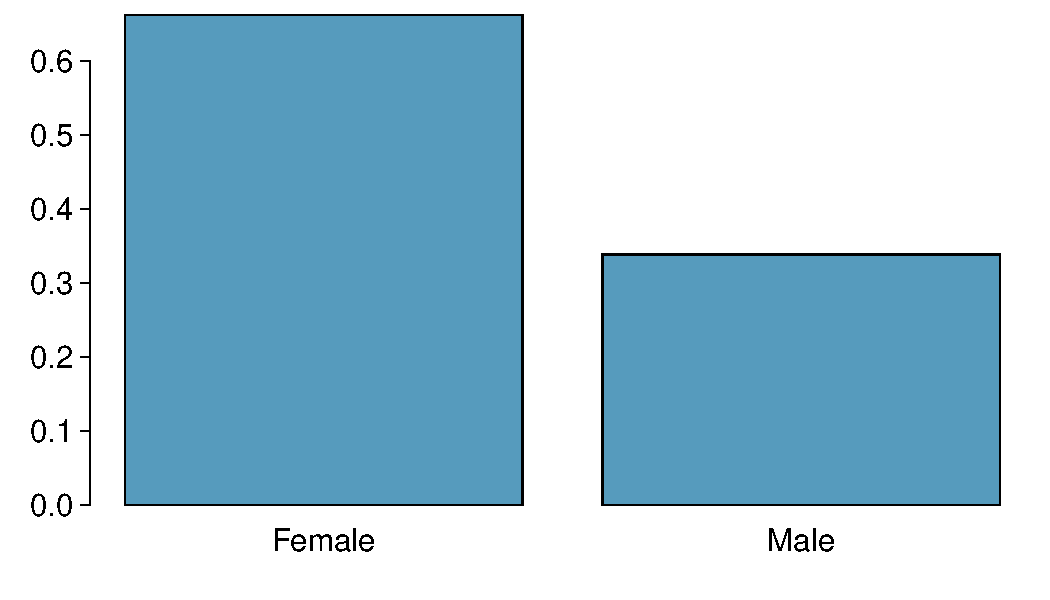
\includegraphics[width=0.4\textwidth]{1-7_categorical_data/figures/gender_spouse/gender_rel_bar}
\end{center}

\pause

\dq{How are bar plots different than histograms?}

\soln{\pause{{\scriptsize Bar plots are used for displaying distributions of categorical variables, while histograms are used for numerical variables. The x-axis in a histogram is a number line,  hence the order of the bars cannot be changed, while in a bar plot the categories can be listed in any order (though some orderings make more sense than others, especially for ordinal variables.)}}}

\end{frame}

%%%%%%%%%%%%%%%%%%%%%%%%%%%%%%%%%%

%%%%%%%%%%%%%%%%%%%%%%%%%%%%%%%%%%%%

\subsection{Row and column proportions}

%%%%%%%%%%%%%%%%%%%%%%%%%%%%%%%%%%%%

\begin{frame}
\frametitle{Choosing the appropriate proportion}

\dq{Does there appear to be a relationship between gender and whether the student is looking for a spouse in college?}

\begin{center}
\begin{tabular}{l l cc r}
					& 			& \multicolumn{2}{c}{{looking for spouse}} \\
  \cline{3-4}
					&			& No	& Yes	& Total \\ 
  \cline{2-5}
\multirow{2}{*}{{gender}}& Female 		& 86 	& 51 		& 137 \\ 
  					& Male 		& 52 	& 18	 	& 70\\ 
  \cline{2-5}
  					& Total		& 138& 69	&  207 \\
  \cline{2-5}
\end{tabular}
\end{center}

\pause

To answer this question we examine the row proportions: 

\pause

\begin{itemize}

\item \% Females looking for a spouse: $51 / 137 \approx 0.37$ \\

\pause

\item \% Males looking for a spouse: $18 / 70 \approx 0.26$ \\

\end{itemize}

\end{frame}

%%%%%%%%%%%%%%%%%%%%%%%%%%%%%%%%%%%%

\subsection{Segmented bar and mosaic plots}

%%%%%%%%%%%%%%%%%%%%%%%%%%%%%%%%%%%%

\begin{frame}
\frametitle{Segmented bar and mosaic plots}

\dq{What are the differences between the three visualizations shown below?}

\begin{center}
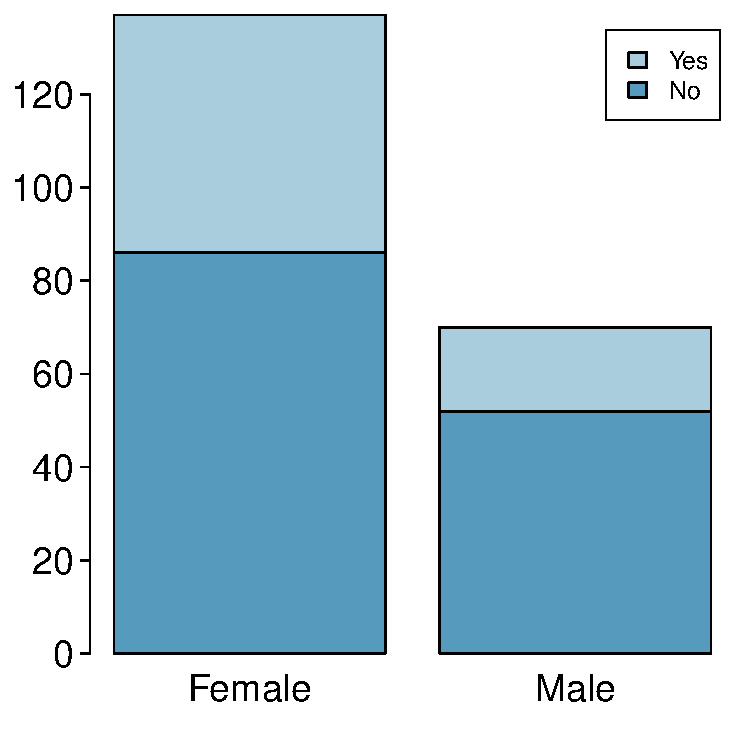
\includegraphics[width=0.30\textwidth]{1-7_categorical_data/figures/gender_spouse/gender_seg_bar}
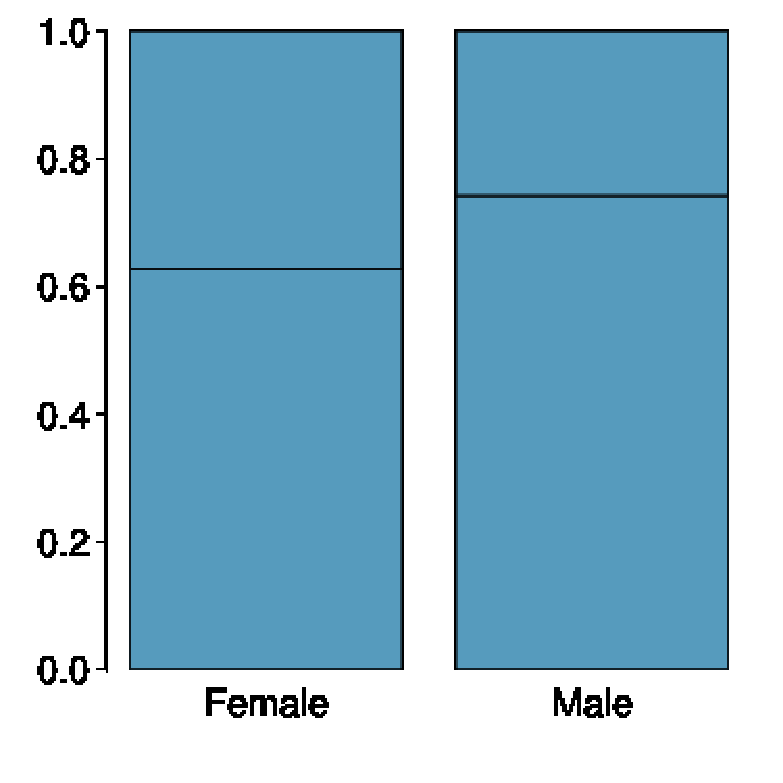
\includegraphics[width=0.30\textwidth]{1-7_categorical_data/figures/gender_spouse/gender_rel_seg_bar}
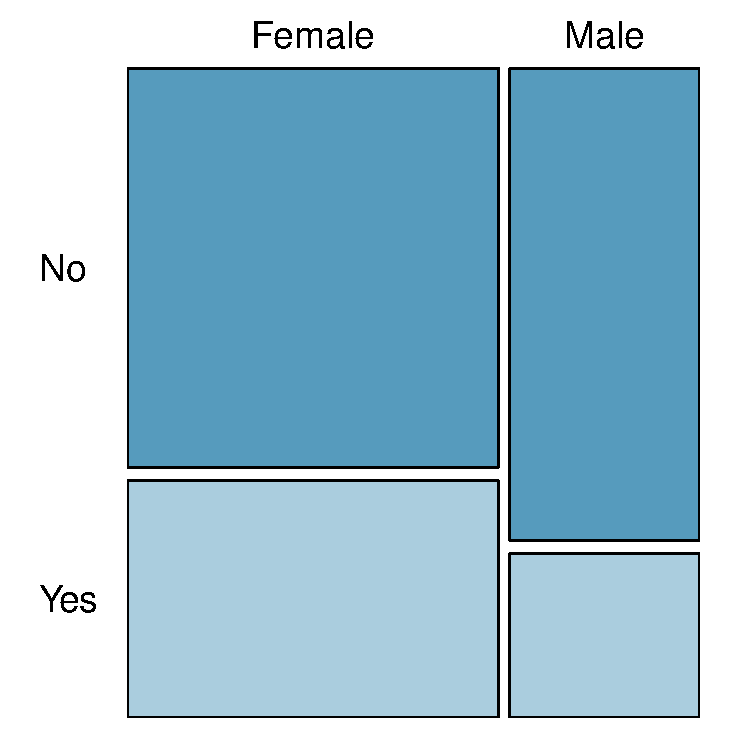
\includegraphics[width=0.30\textwidth]{1-7_categorical_data/figures/gender_spouse/gender_mosaic}
\end{center}

\end{frame}




%%%%%%%%%%%%%%%%%%%%%%%%%%%%%%%%%%%%

\subsection{Example: Marbles}

%%%%%%%%%%%%%%%%%%%%%%%%%%%%%%%%%%%%

\begin{frame}
\frametitle{Example: Marbles}

Imagine an urn contains 100 marbles, each having a color and a pattern. The colors are green, violet, and blue. The patterns are checkered, dotted, and striped. The frequencies (counts) are shown in the contingency table.

\begin{center}
\begin{tabular}{c|c c c | c}
       & checkered & dotted & striped & total \\ \hline
green  &  20       &  18    & 21 & 59 \\
violet & 8         &  9     & 3  & 20 \\
blue   & 12        & 3      & 6  & 21 \\ \hline
total  & 40        & 30     & 30 & 100 
\end{tabular}
\end{center}

There are a variety of interesting proportions: simple part of whole, compound part of whole, and part of part.

\end{frame}

%%%%%%%%%%%%%%%%%%%%%%%%%%%%%%%%%%%%

\subsection{Example: Marbles - Simple (Marginal) Proportions}

%%%%%%%%%%%%%%%%%%%%%%%%%%%%%%%%%%%%


\begin{frame}
\frametitle{Marbles - Simple (Marginal) Proportions}

\begin{center}
\begin{tabular}{c|c c c | c}
       & checkered & dotted & striped & total \\ \hline
green  &  20       &  18    & 21 & 59 \\
violet & 8         &  9     & 3  & 20 \\
blue   & 12        & 3      & 6  & 21 \\ \hline
total  & 40        & 30     & 30 & 100 
\end{tabular}
\end{center}

Simple part of whole:
\begin{itemize}
\item What proportion of marbles are checkered? \soln{\pause $\frac{40}{100}=0.40$}
\item What proportion of marbles are green? \soln{\pause $\frac{59}{100}=0.59$}
\item What proportion of marbles are striped? \soln{\pause $\frac{30}{100}=0.30$}
\item What proportion of marbles are blue? \soln{\pause $\frac{21}{100}=0.21$}
\end{itemize}

\end{frame}


%%%%%%%%%%%%%%%%%%%%%%%%%%%%%%%%%%%%

\subsection{Example: Marbles - Compound Proportions}

%%%%%%%%%%%%%%%%%%%%%%%%%%%%%%%%%%%%


\begin{frame}
\frametitle{Marbles - Compound Proportions}

\begin{center}
\begin{tabular}{c|c c c | c}
       & checkered & dotted & striped & total \\ \hline
green  &  20       &  18    & 21 & 59 \\
violet & 8         &  9     & 3  & 20 \\
blue   & 12        & 3      & 6  & 21 \\ \hline
total  & 40        & 30     & 30 & 100 
\end{tabular}
\end{center}

Compound part of whole:
\begin{itemize}
\item What proportion of marbles are dotted and violet? \soln{\pause $\frac{9}{100}=0.09$}
\item What proportion of marbles are green and striped? \soln{\pause $\frac{21}{100}=0.21$}
\item What proportion of marbles are green or striped? \soln{\pause $\frac{20+18+21+3+6}{100}=0.68$}
\item What proportion of marbles are dotted or violet? \soln{\pause $\frac{30+20-9}{100}=0.41$}
\end{itemize}

\end{frame}


%%%%%%%%%%%%%%%%%%%%%%%%%%%%%%%%%%%%

\subsection{Example: Marbles - Conditional Proportions}

%%%%%%%%%%%%%%%%%%%%%%%%%%%%%%%%%%%%


\begin{frame}
\frametitle{Marbles - Conditional Proportions}

\begin{center}
\begin{tabular}{c|c c c | c}
       & checkered & dotted & striped & total \\ \hline
green  &  20       &  18    & 21 & 59 \\
violet & 8         &  9     & 3  & 20 \\
blue   & 12        & 3      & 6  & 21 \\ \hline
total  & 40        & 30     & 30 & 100 
\end{tabular}
\end{center}

Part of part:
\begin{itemize}
\item What proportion of violet marbles are dotted? \soln{\pause $\frac{9}{20}=0.45$}
\item What proportion of dotted marbles are violet? \soln{\pause $\frac{9}{30}=0.30$}
\item What proportion of green marbles are striped? \soln{\pause $\frac{21}{59}\approx 0.356$}
\item What proportion of striped marbles are green? \soln{\pause $\frac{21}{30}=0.70$}
\end{itemize}

\end{frame}


%%%%%%%%%%%%%%%%%%%%%%%%%%%%%%%%%%%%

\subsection{Example: Marbles - Mosaic Plot}

%%%%%%%%%%%%%%%%%%%%%%%%%%%%%%%%%%%%


\begin{frame}
\frametitle{Marbles - Mosaic Plot}

\tiny
\begin{tabular}{c|c c c | c}
       & checkered & dotted & striped & total \\ \hline
green  &  20       &  18    & 21 & 59 \\
violet & 8         &  9     & 3  & 20 \\
blue   & 12        & 3      & 6  & 21 \\ \hline
total  & 40        & 30     & 30 & 100 
\end{tabular}
\begin{center}
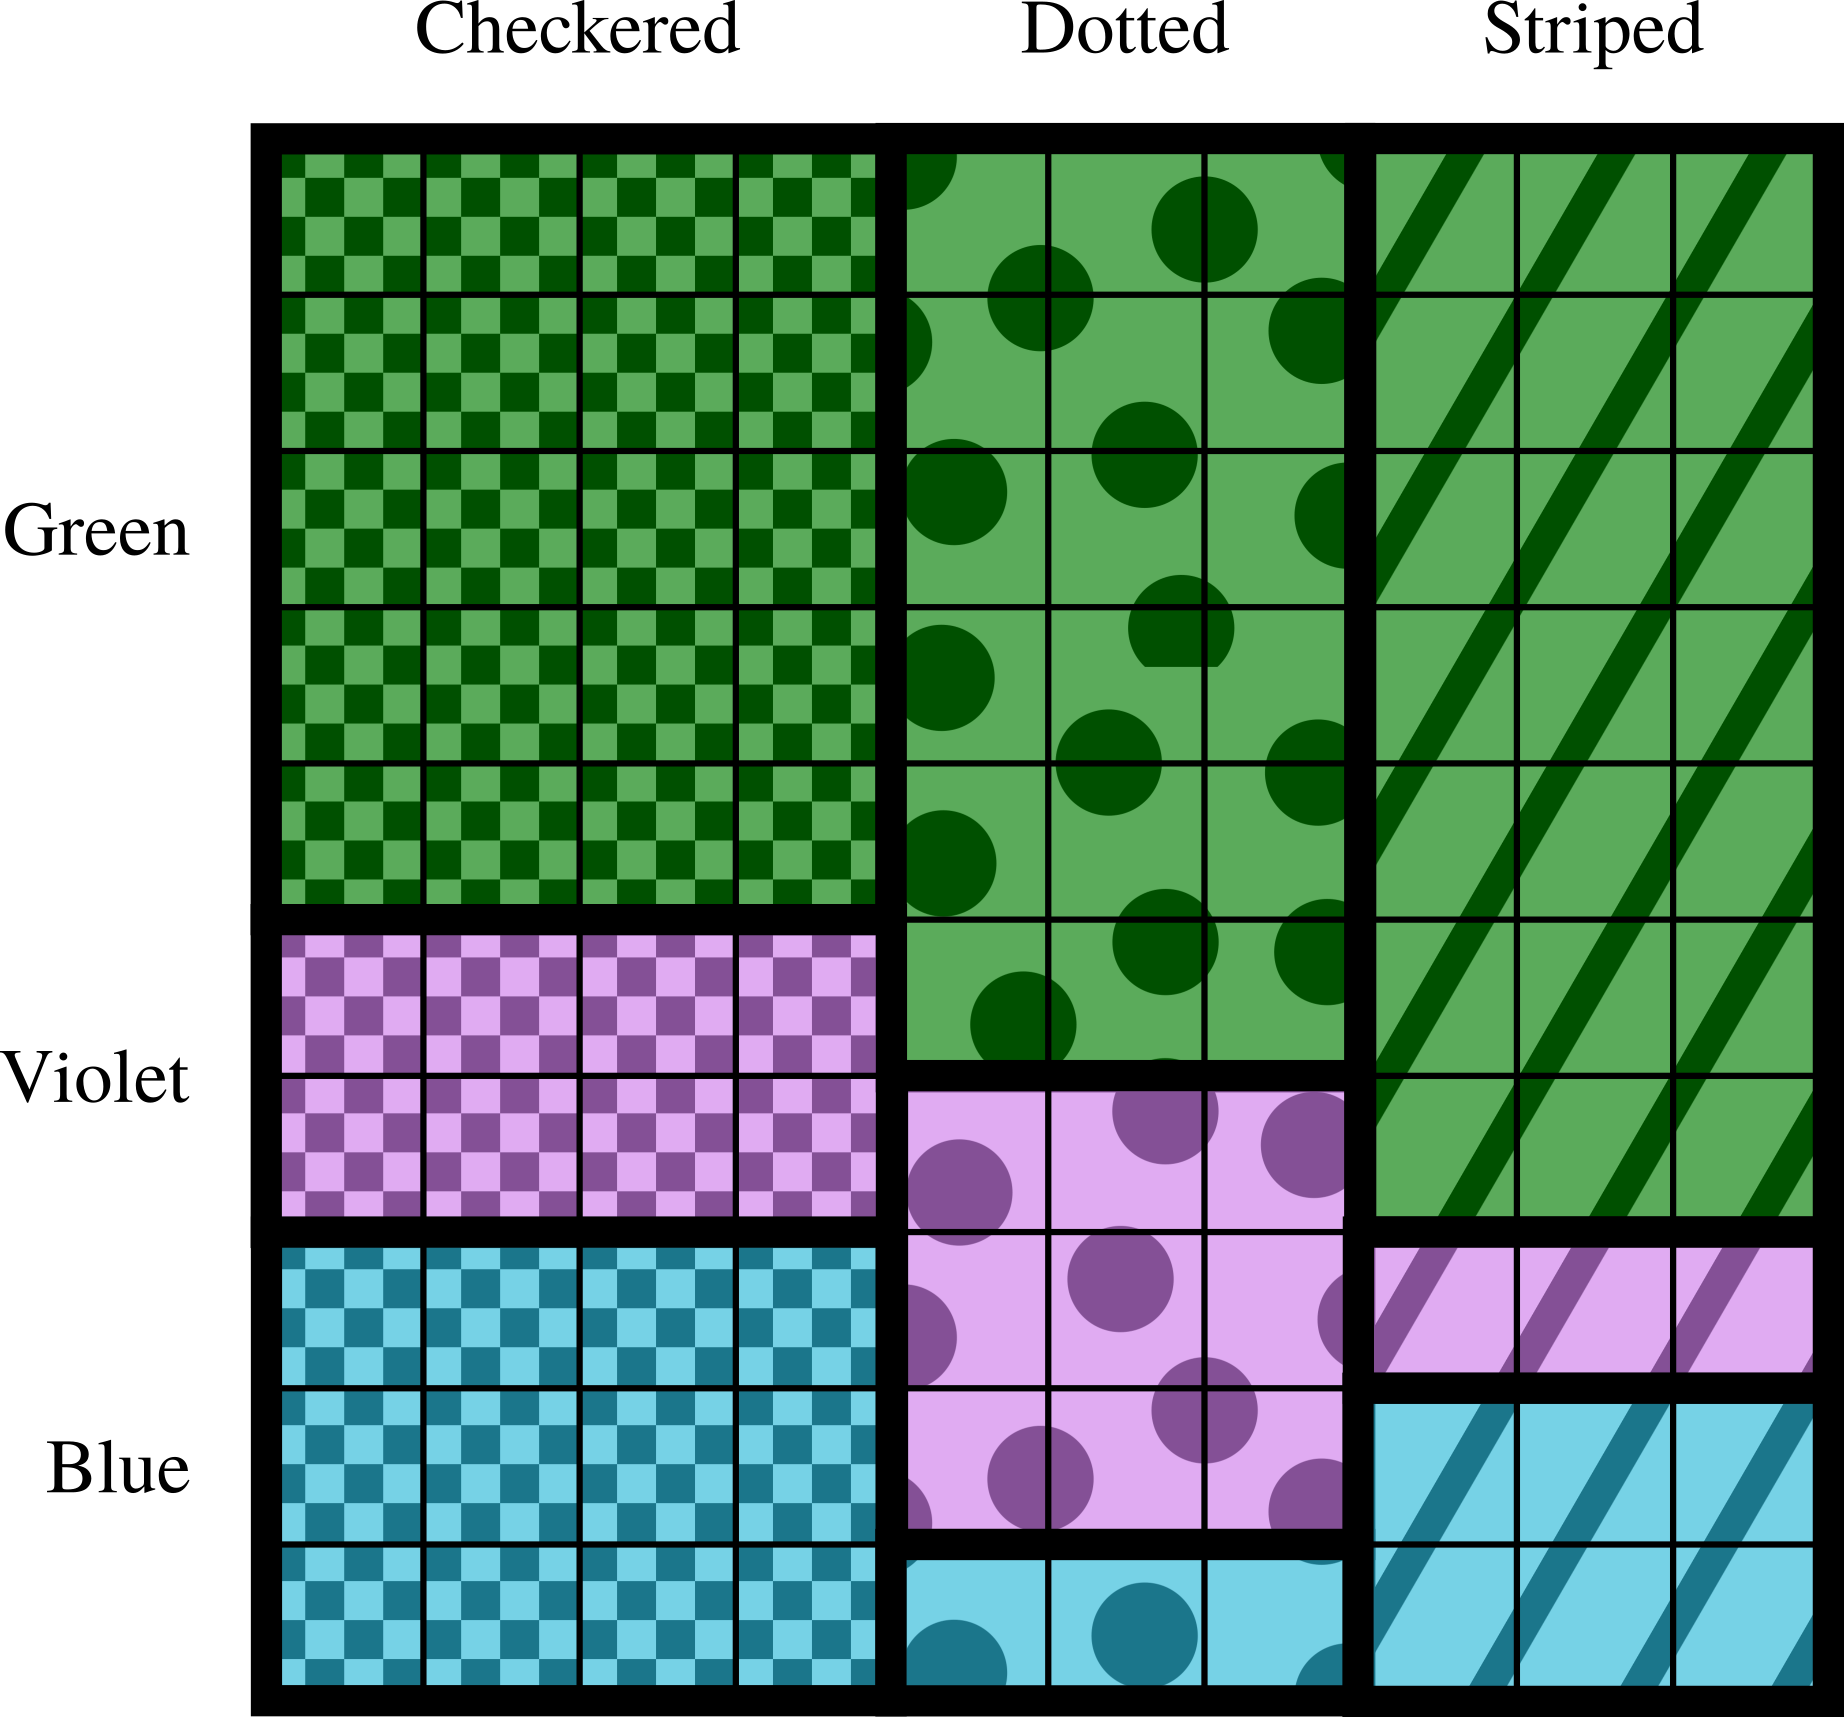
\includegraphics[scale=0.4]{1-7_categorical_data/figures/mosaic/mosaic5.png}
\end{center}


\end{frame}

%%%%%%%%%%%%%%%%%%%%%%%%%%%%%%%%%%%%%

%\subsection{Example: Marbles - Making a Mosaic Plot}

%%%%%%%%%%%%%%%%%%%%%%%%%%%%%%%%%%%%%


\begin{frame}
\frametitle{Marbles - Making a Mosaic Plot}
\small
\begin{enumerate}
\item Start with a rectangle (a square is good).
\end{enumerate}
\\ \vfill
\begin{center}
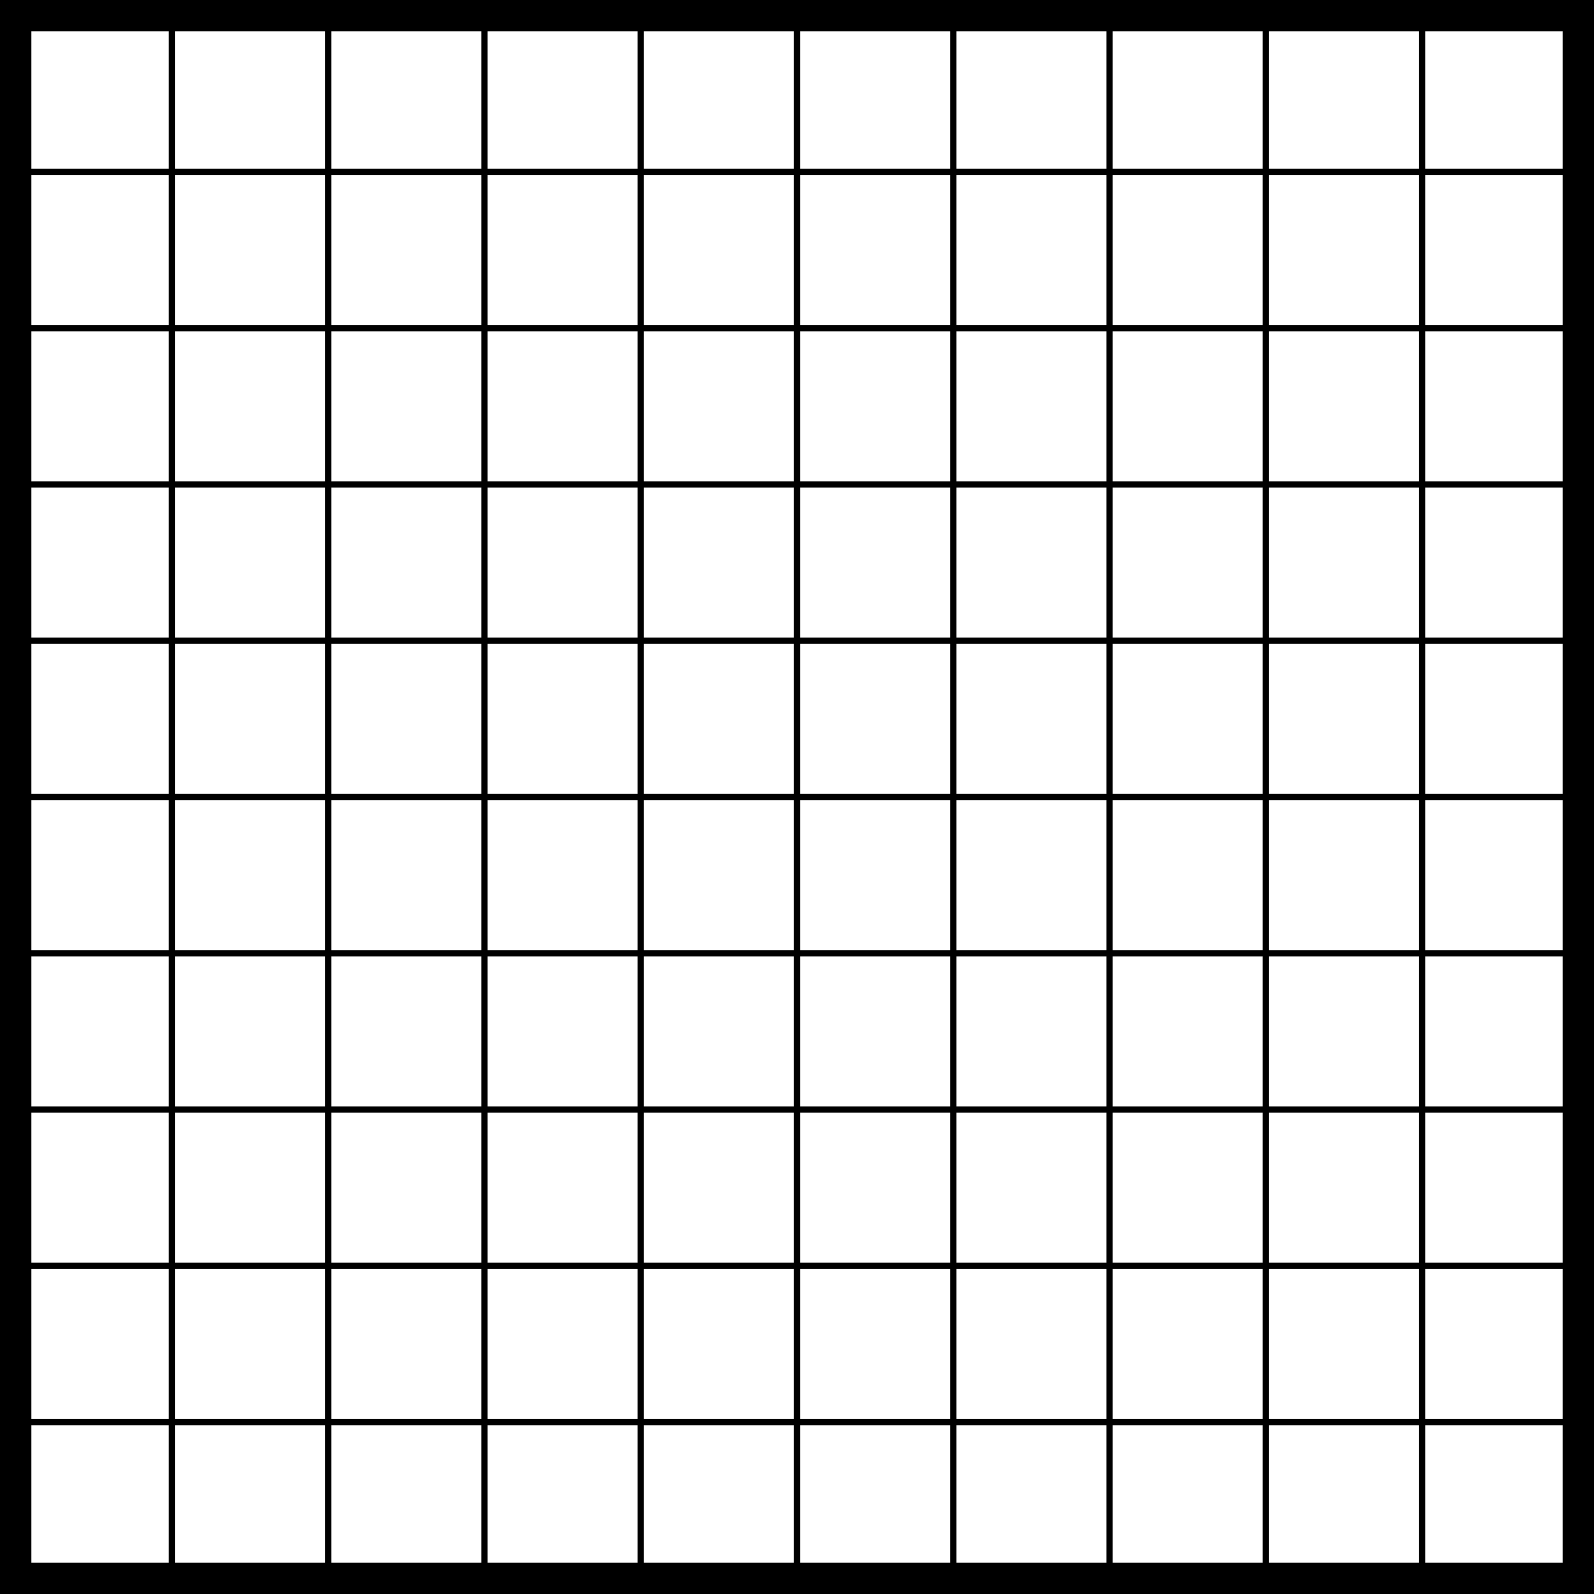
\includegraphics[scale=0.3]{1-7_categorical_data/figures/mosaic/square.png}
\end{center}
\end{frame}

\begin{frame}
\small
\begin{enumerate}
\item Start with a rectangle (a square is good).
\item Find marginal proportions of first variable for widths of columns.
\end{enumerate}
\begin{center}
$\frac{40}{100} = 0.4 $, $\frac{30}{100} = 0.3 $, $\frac{30}{100} = 0.3 $
\end{center}
\\\vfill
\begin{center}
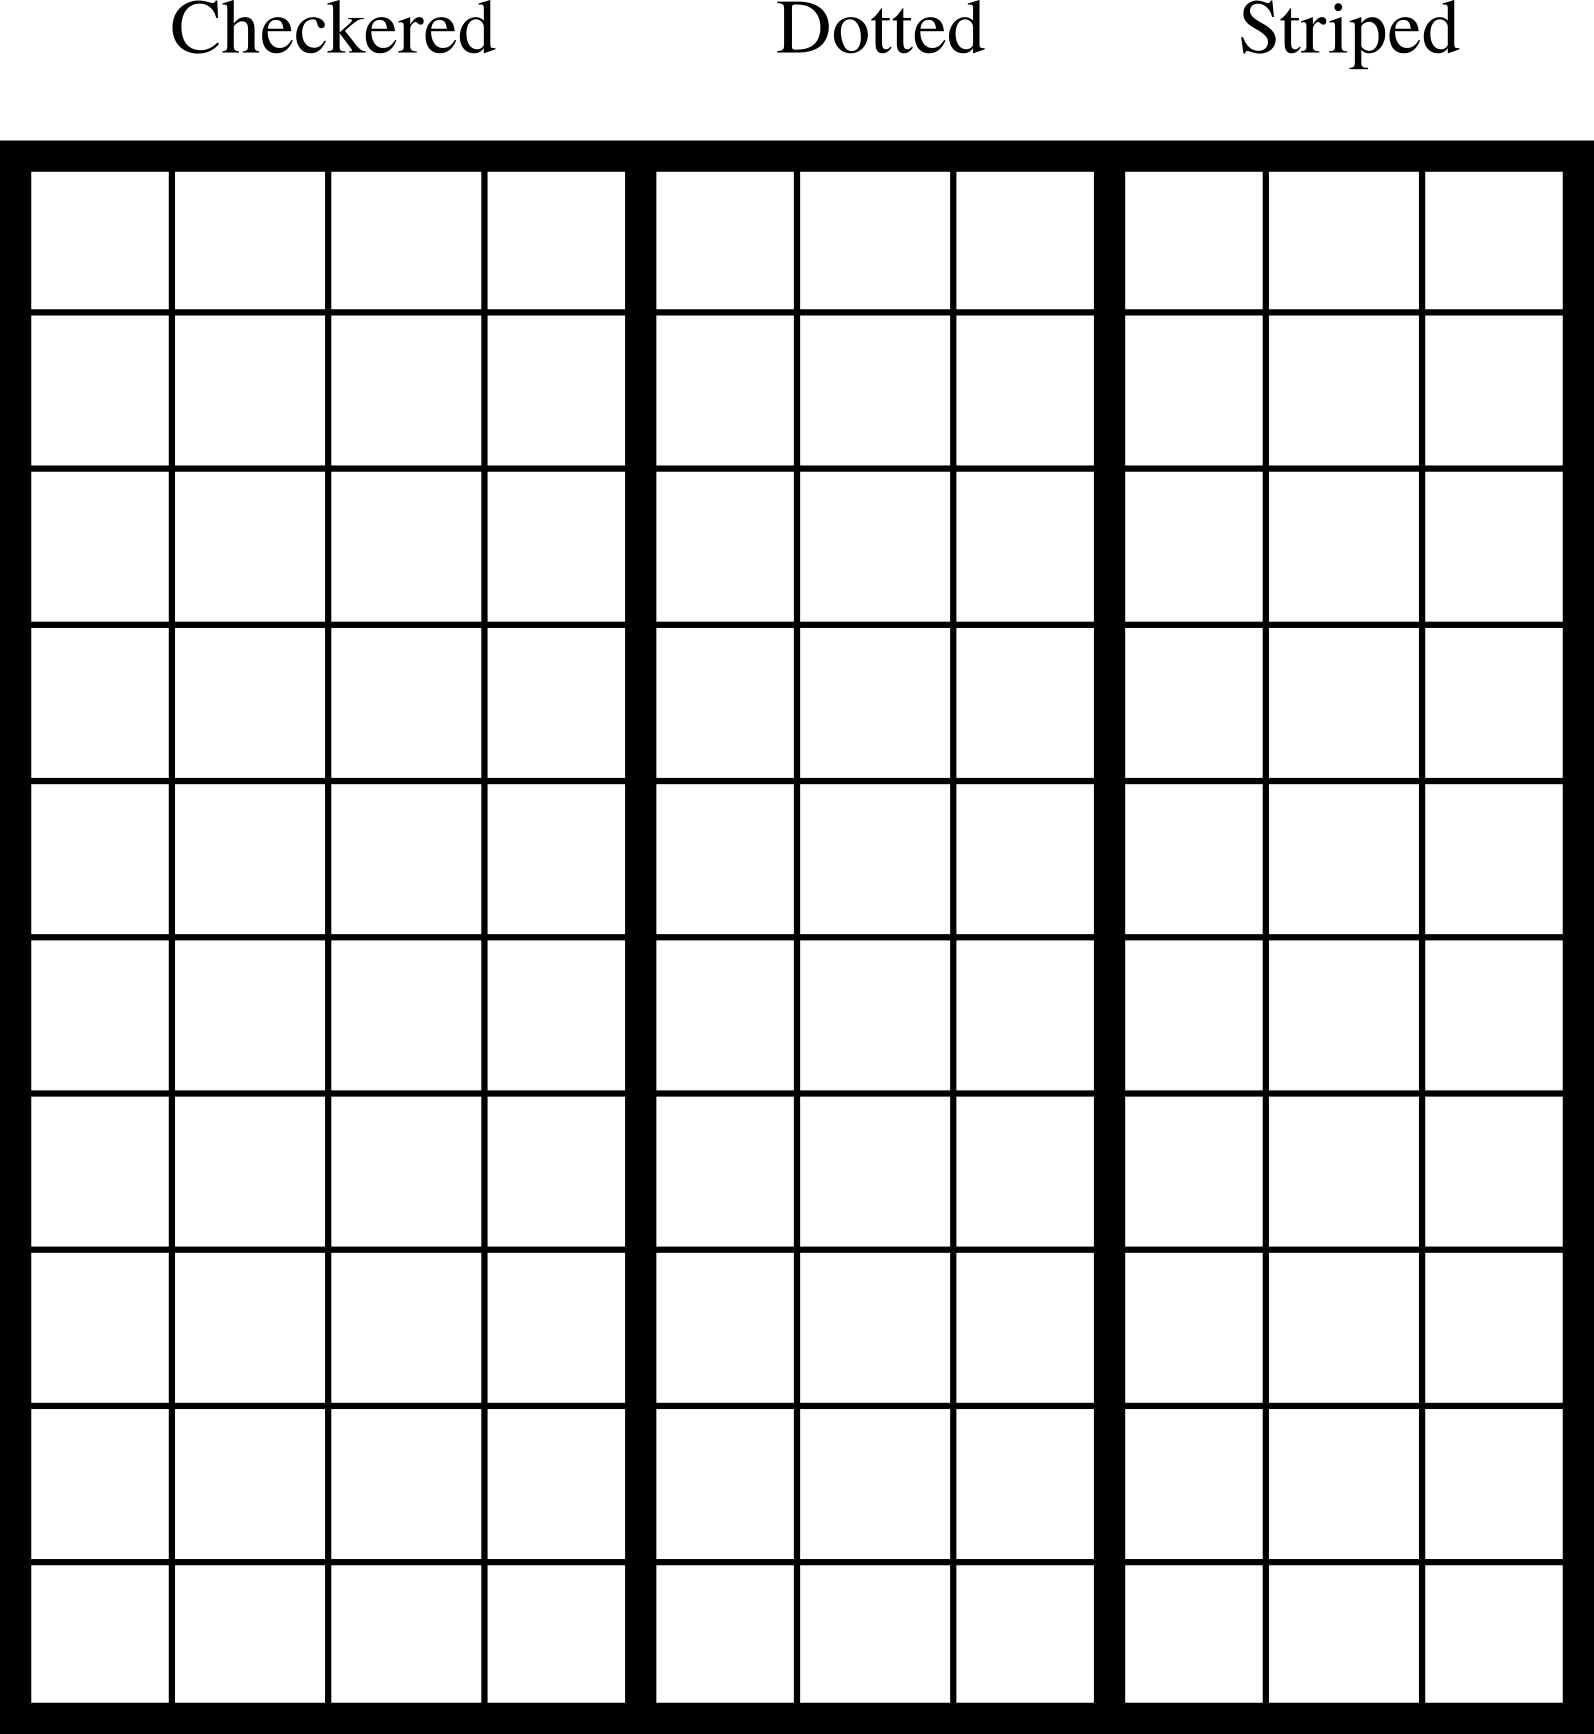
\includegraphics[scale=0.3]{1-7_categorical_data/figures/mosaic/cols.png}
\end{center}
\end{frame}

\begin{frame}
\small
\begin{enumerate}
\item Start with a rectangle (a square is good).
\item Find marginal proportions of first variable for widths of columns.
\item For heights of rectangles, determine part-of-part proportions, e.g. the proportion of checkered marbles that are green.
\end{enumerate}
\begin{center}
\begin{tabular}{c c c}
$\frac{20}{40} = 0.5$ &  $\frac{18}{30} = 0.6$ & $\frac{21}{30} = 0.7$ \\
$\frac{8}{40} = 0.2$ &  $\frac{9}{30} = 0.3$ & $\frac{3}{30} = 0.1$ \\
$\frac{12}{40} = 0.3$ &  $\frac{3}{30} = 0.1$ & $\frac{6}{30} = 0.2$ \\
\end{tabular}
\end{center}
\\ \vfill
\begin{center}
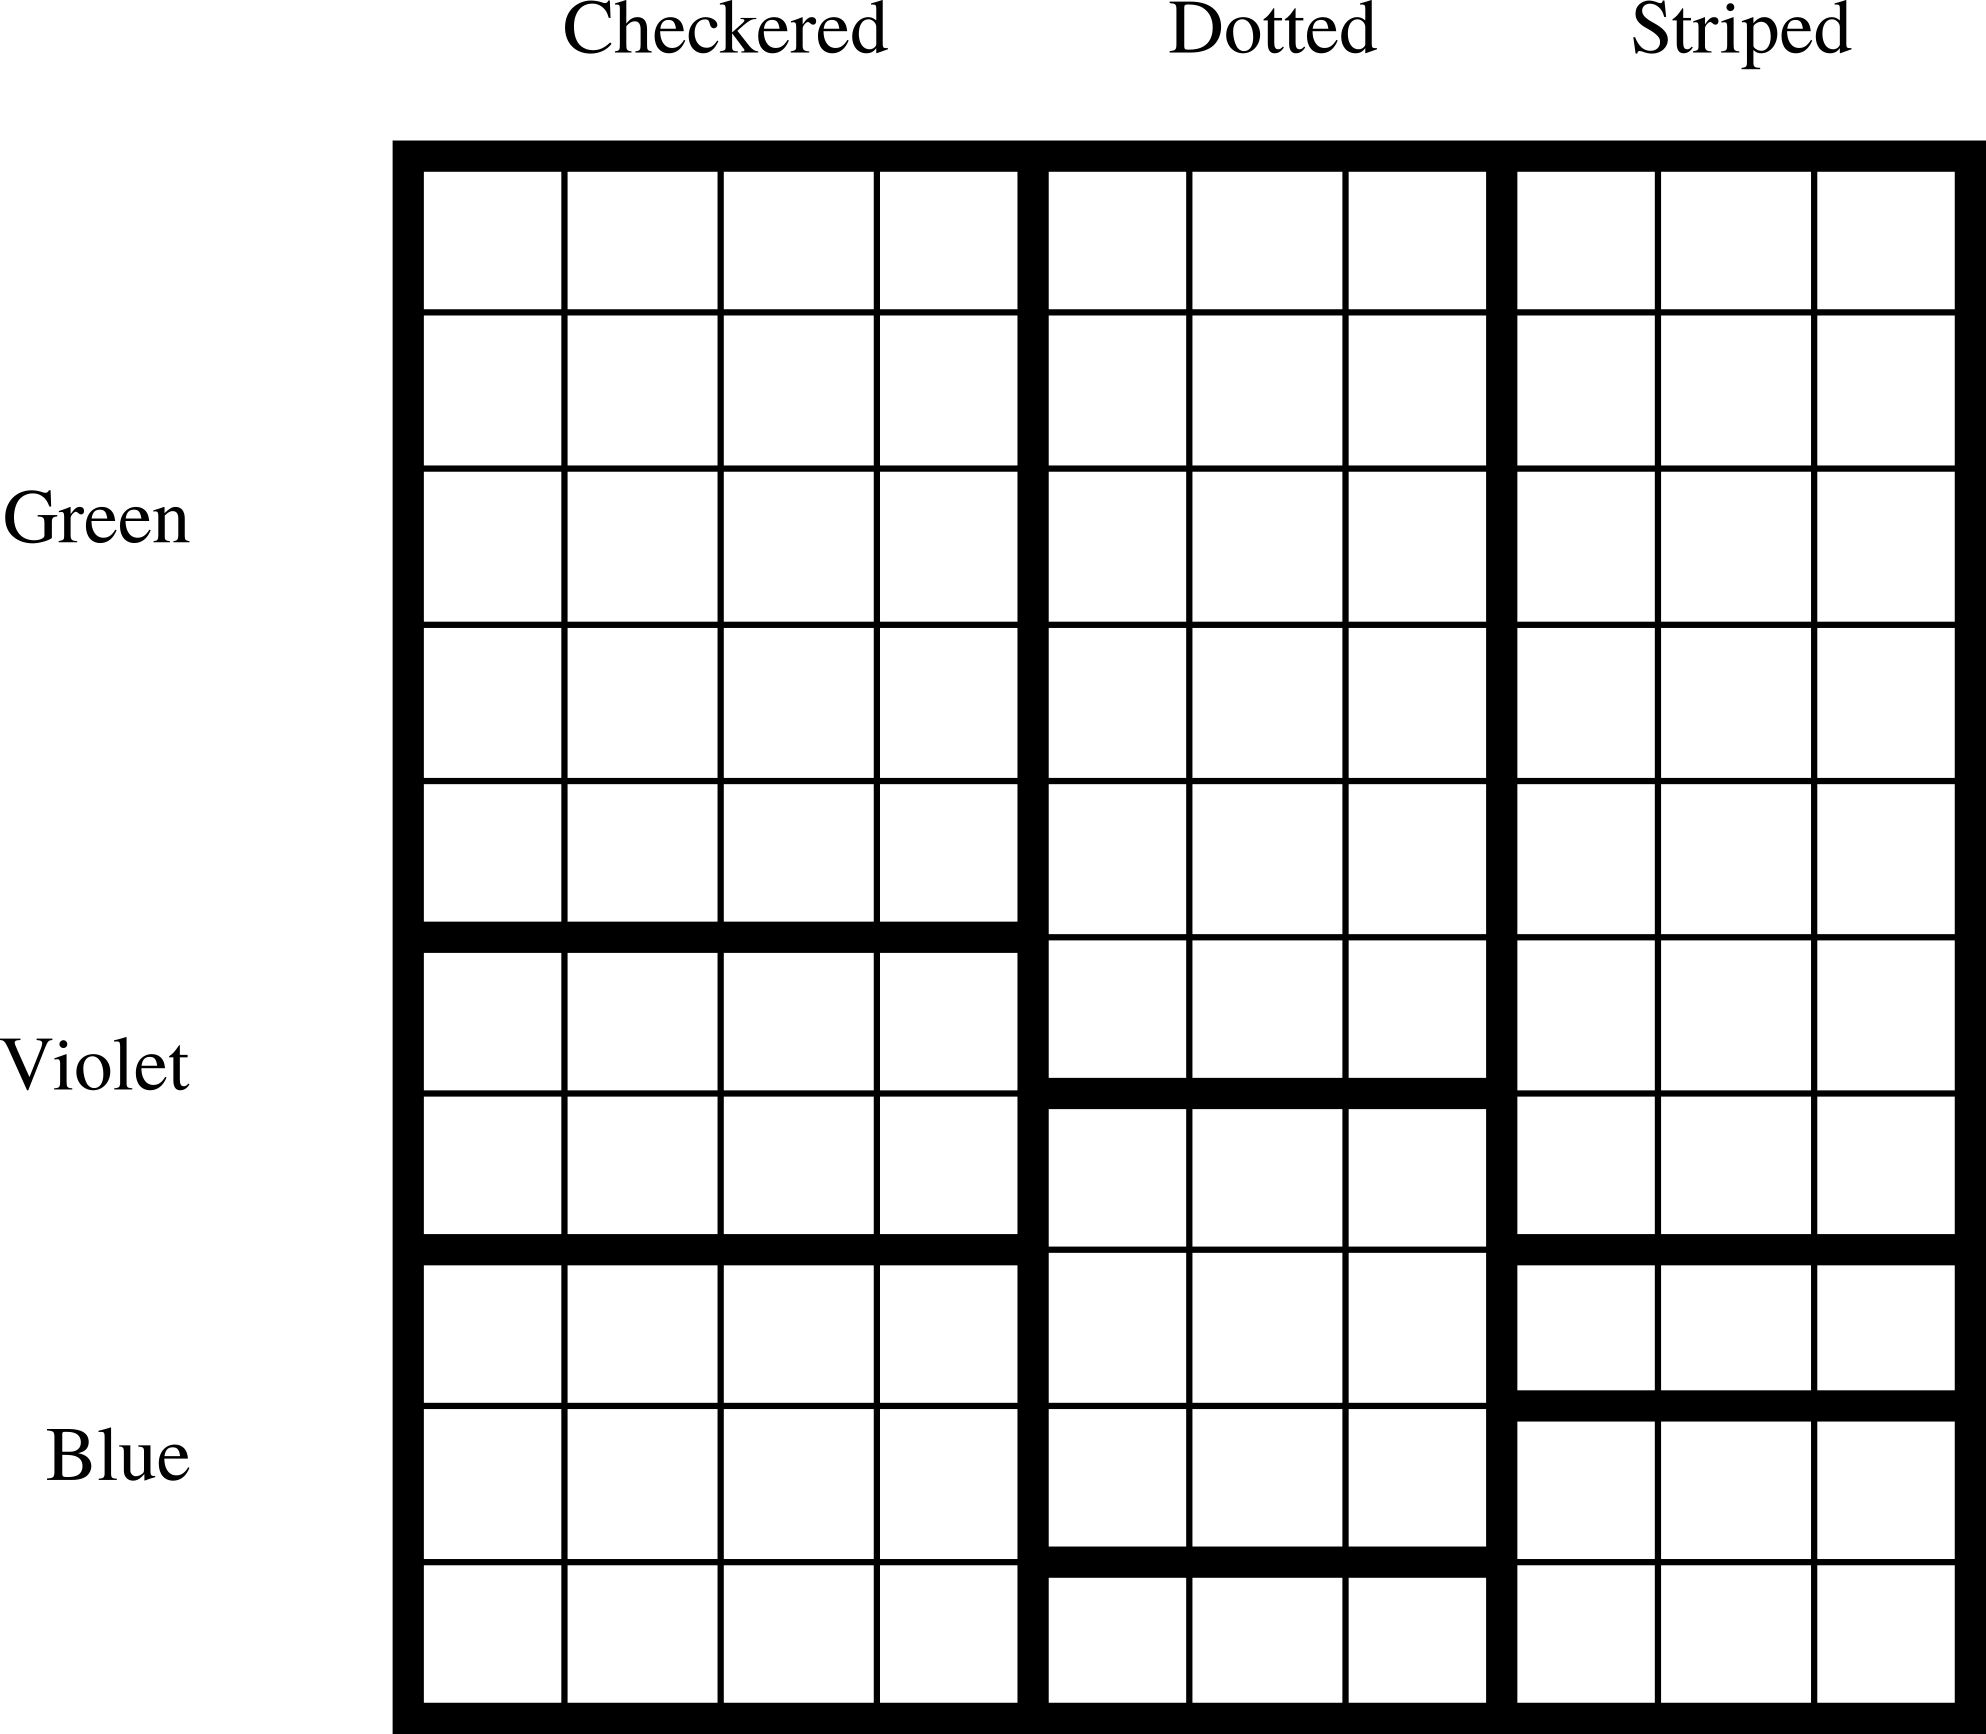
\includegraphics[scale=0.3]{1-7_categorical_data/figures/mosaic/unshaded.png}
\end{center}
\end{frame}

\begin{frame}
\small
\begin{enumerate}
\item Start with a rectangle (a square is good).
\item Find marginal proportions of first variable for widths of columns.
\item For heights of rectangles, determine part-of-part proportions, e.g. the proportion of checkered marbles that are green.
\item Shade according to second variable.
\end{enumerate}
\\ \vfill
\begin{center}
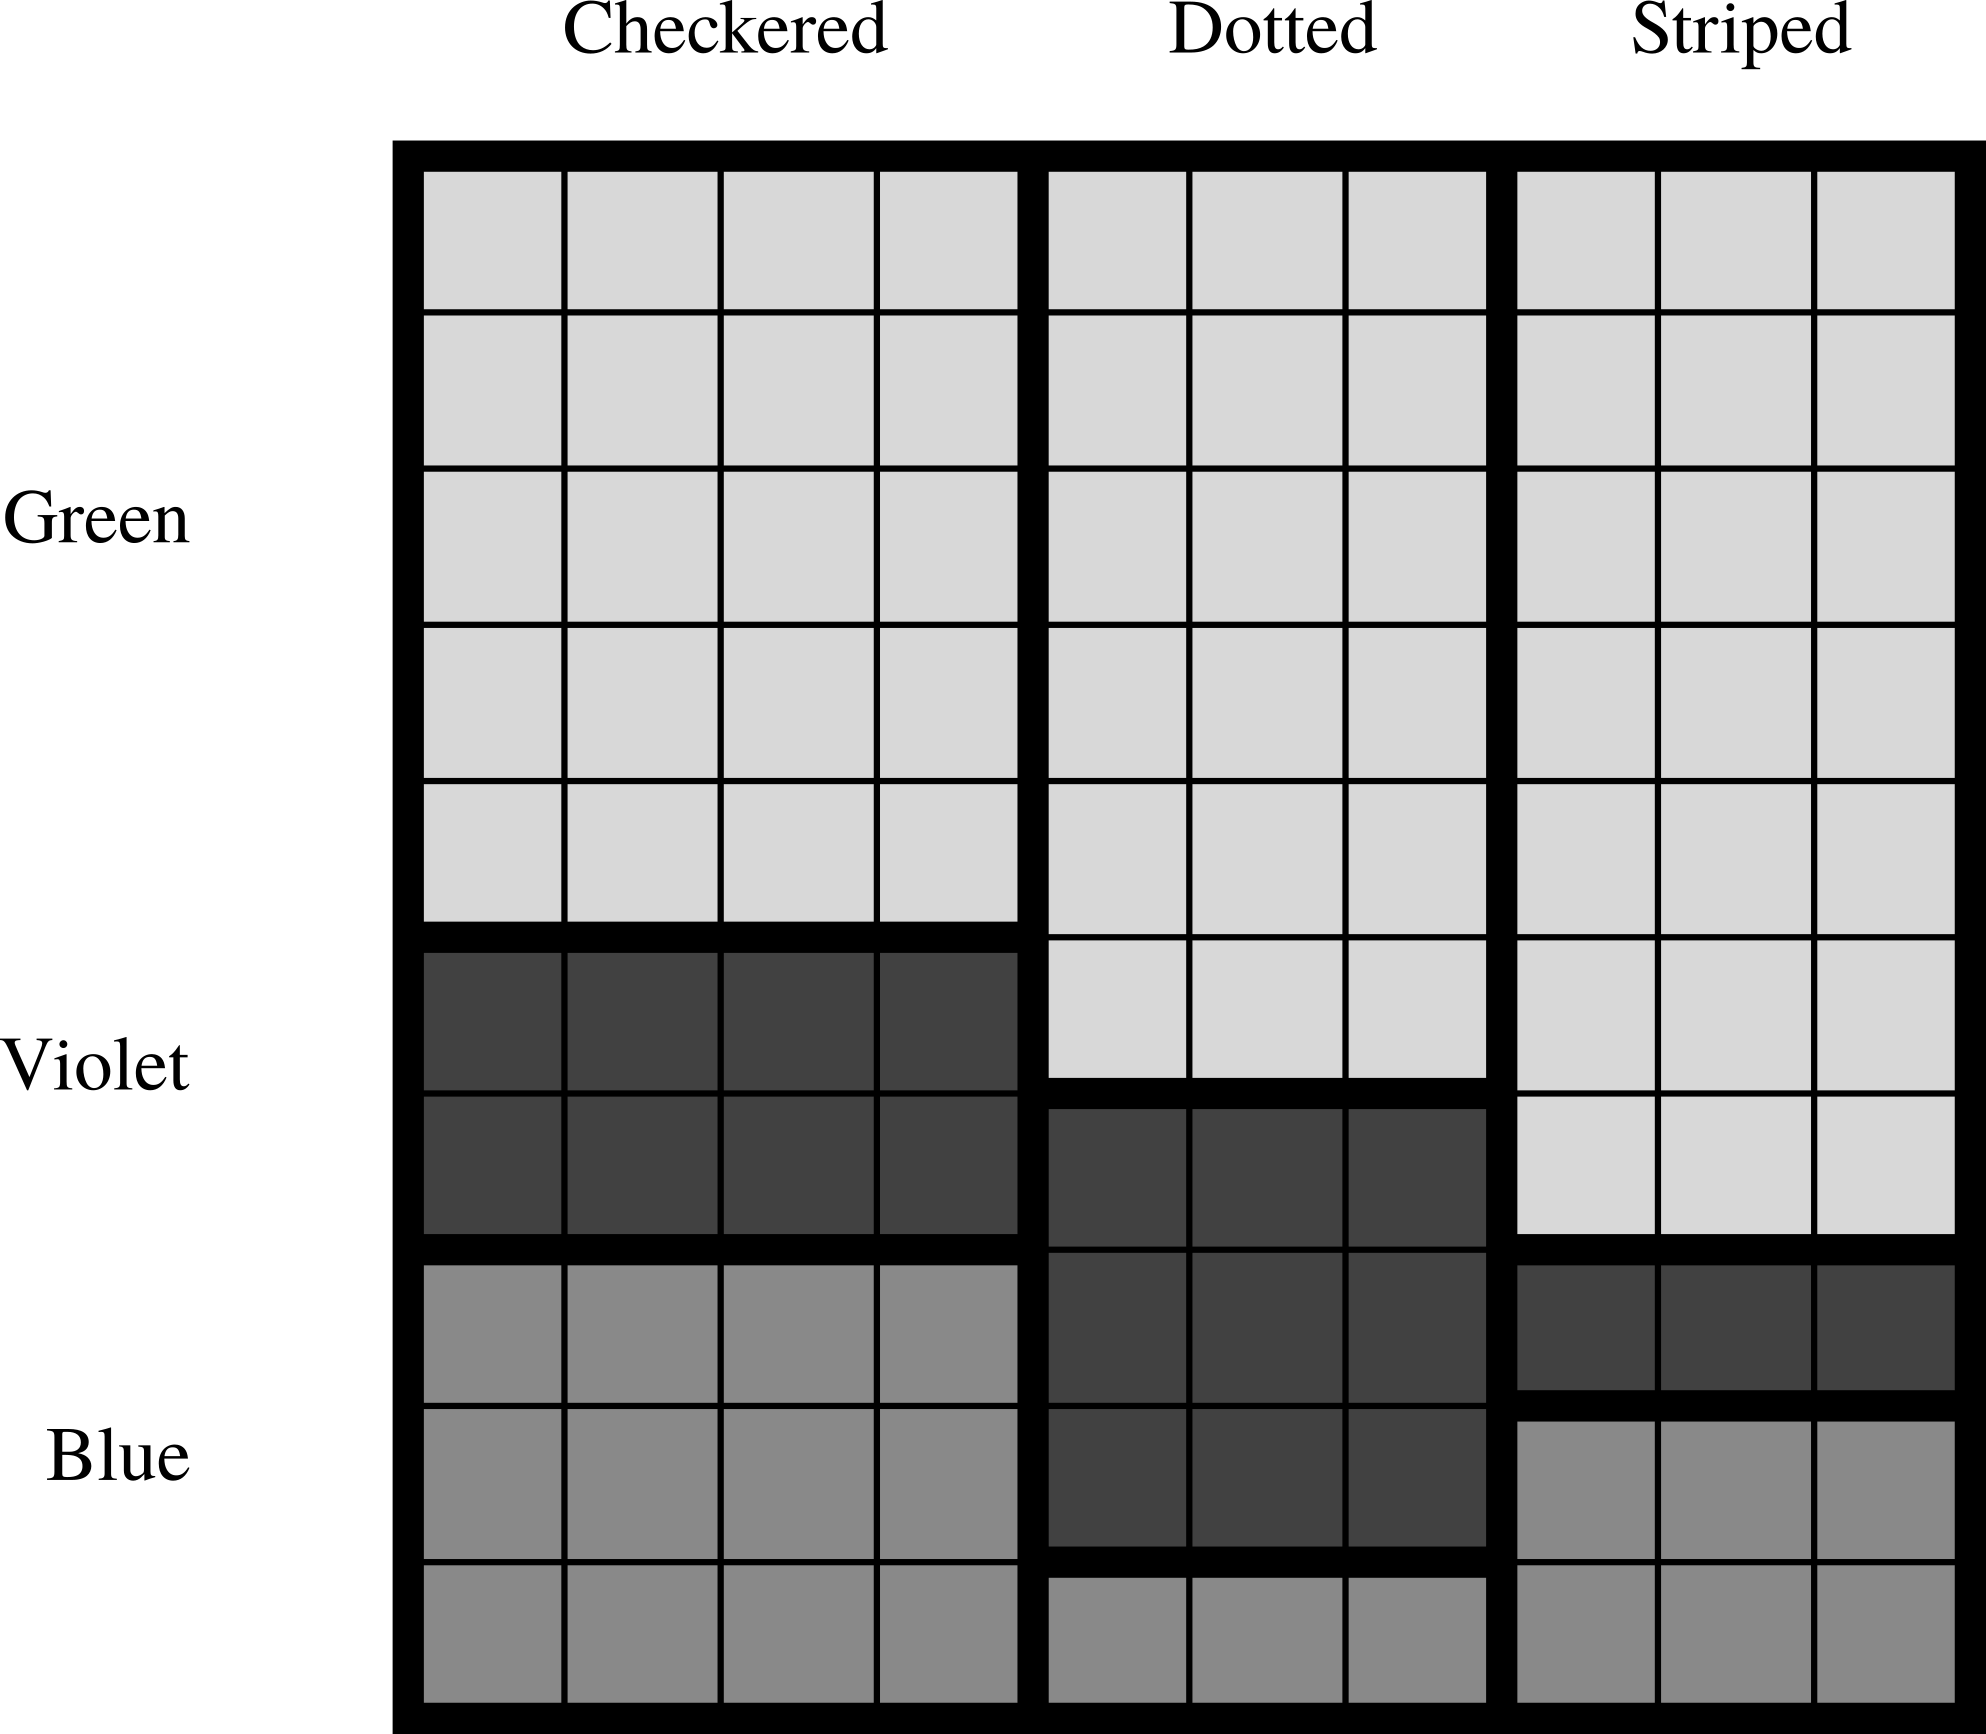
\includegraphics[scale=0.3]{1-7_categorical_data/figures/mosaic/shaded.png}
\end{center}
\end{frame}

%%%%%%%%%%%%%%%%%%%%%%%%%%%%%%%%%%%%

\subsection{Independence in Mosaic Plots}

%%%%%%%%%%%%%%%%%%%%%%%%%%%%%%%%%%%%


\begin{frame}
\frametitle{Independence in Mosaic Plots}

If the two variables are independent, then a mosaic plot's horizontal lines will be continuous (unbroken).
\begin{center}
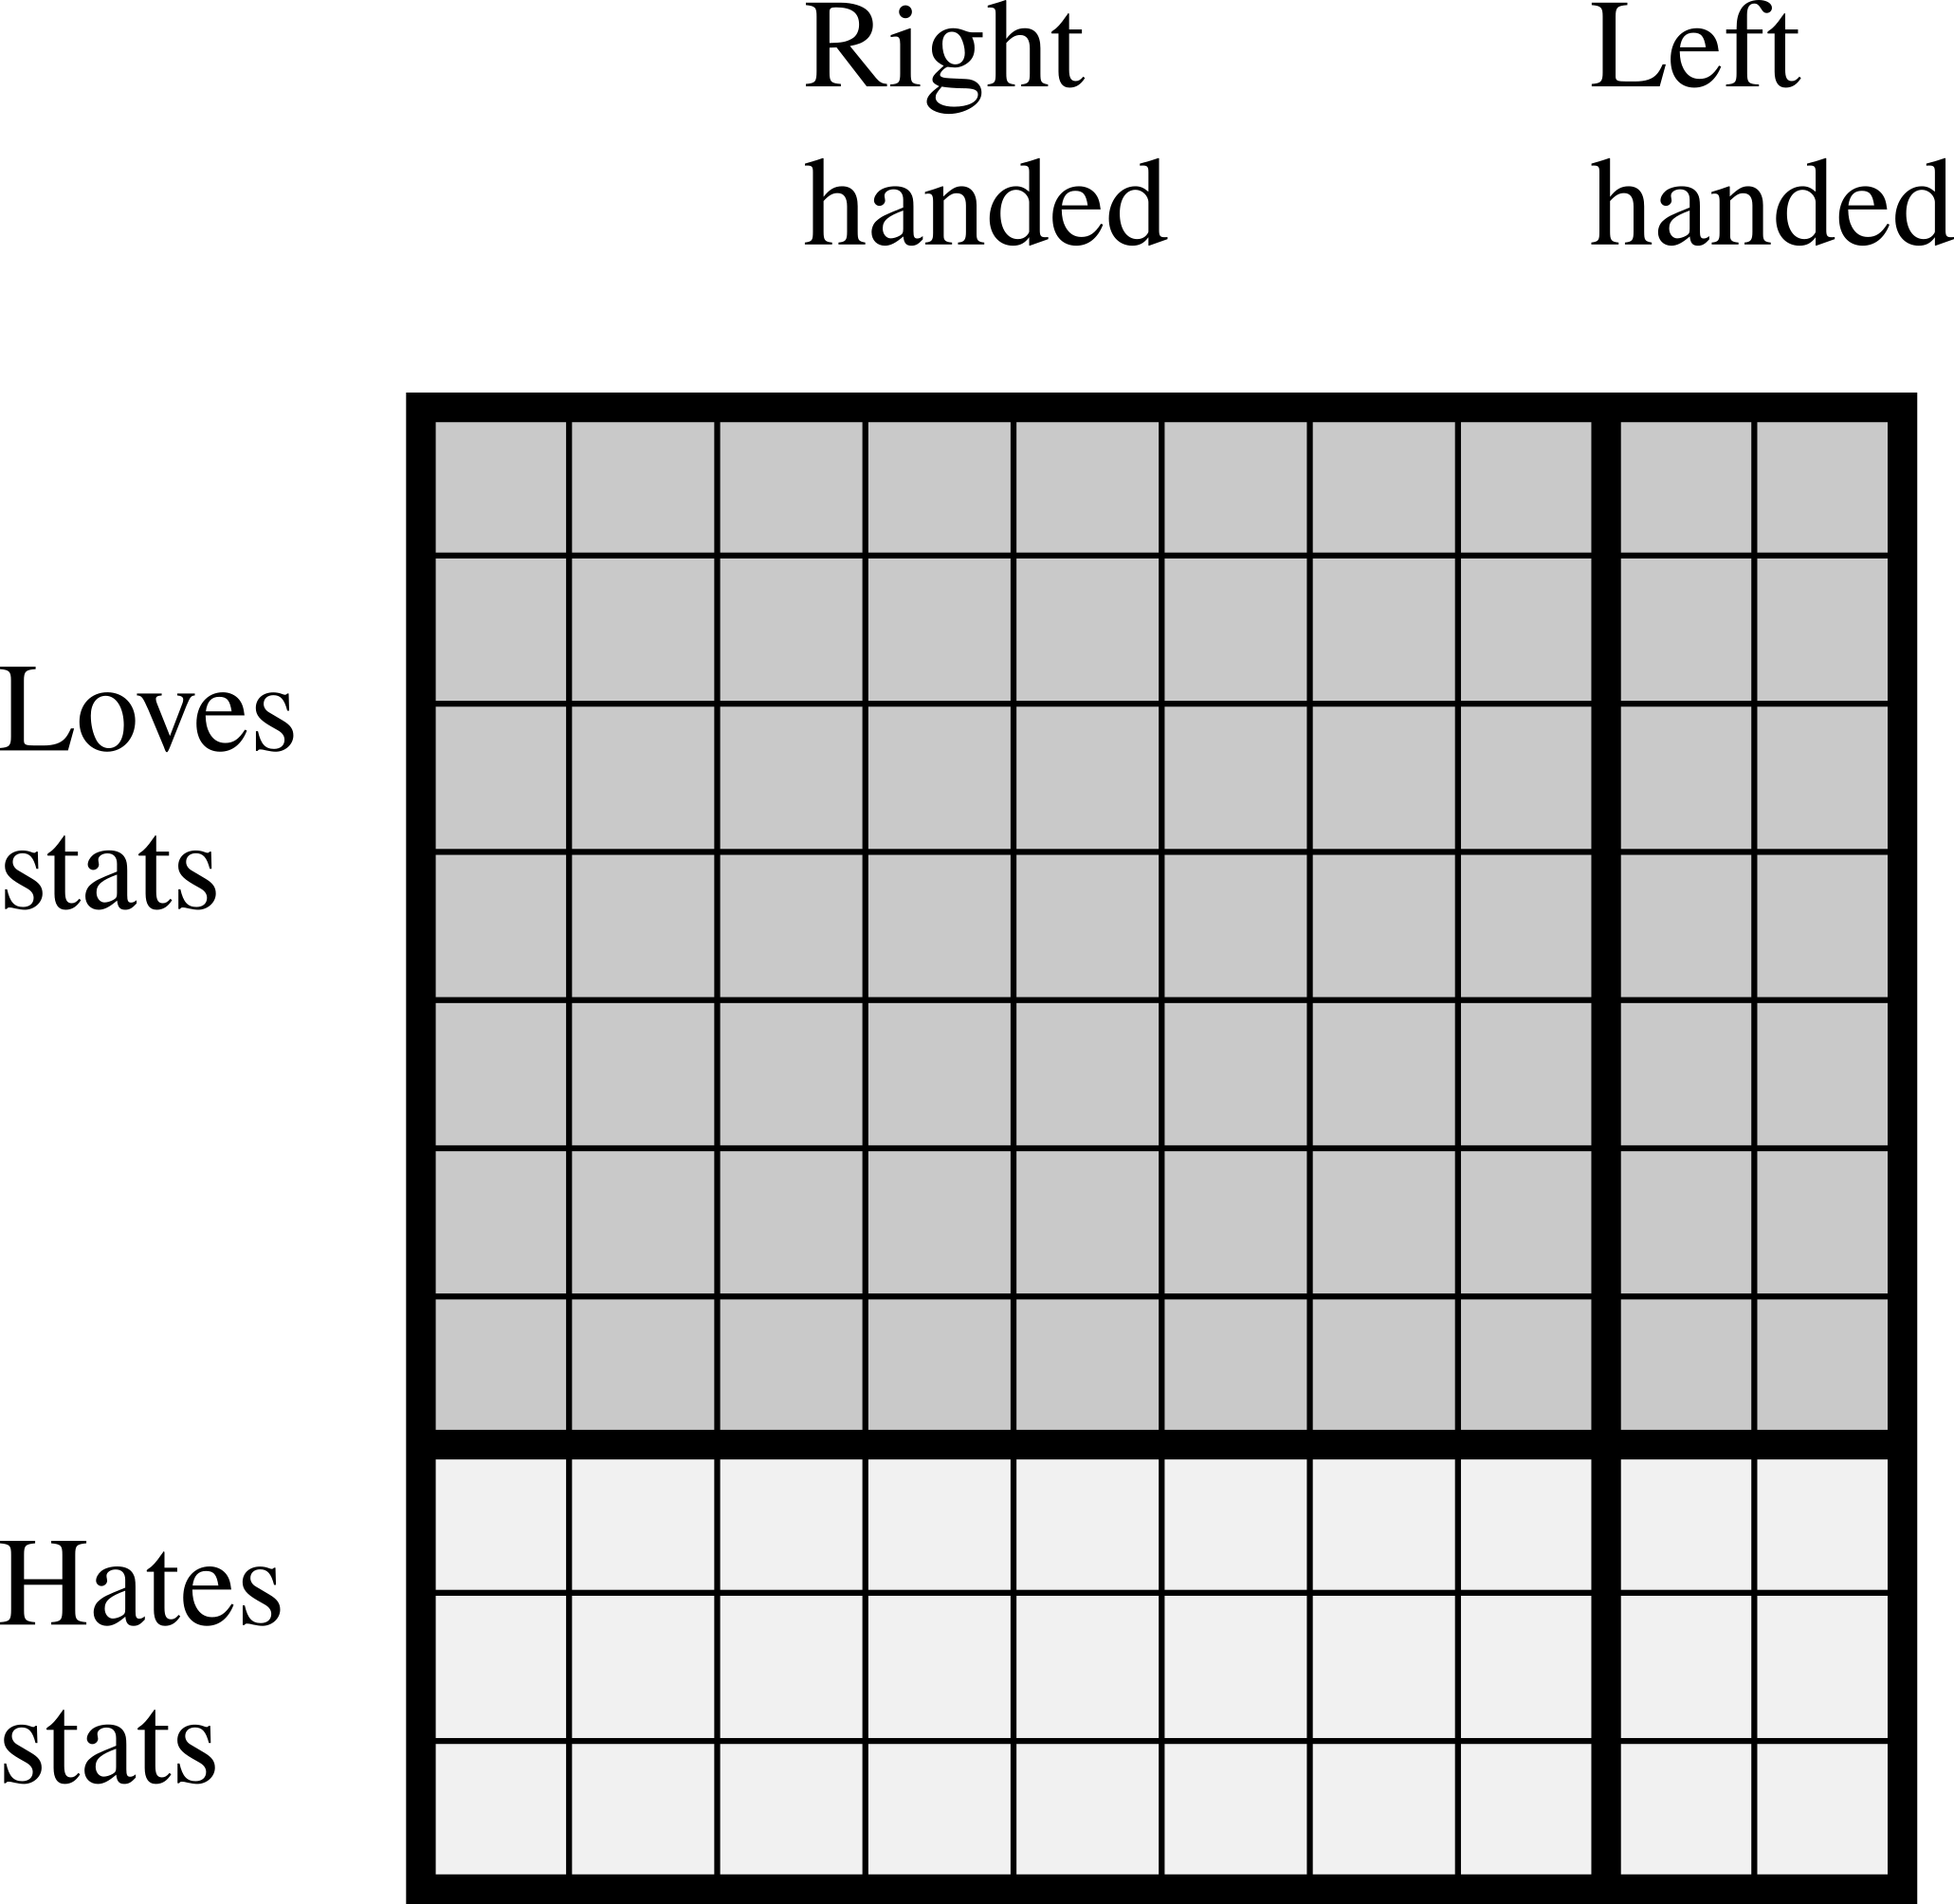
\includegraphics[scale=0.3]{1-7_categorical_data/figures/mosaic/handed.png}
\end{center}


\end{frame}

%%%%%%%%%%%%%%%%%%%%%%%%%%%%%%%%%%%%

%\subsection{Pie charts}

%%%%%%%%%%%%%%%%%%%%%%%%%%%%%%%%%%%%%

%\begin{frame}
%\frametitle{Pie charts}

%\dq{Can you tell which order encompasses the lowest percentage of mammal species?}

%\vspace{-0.5cm}

%\begin{center}
%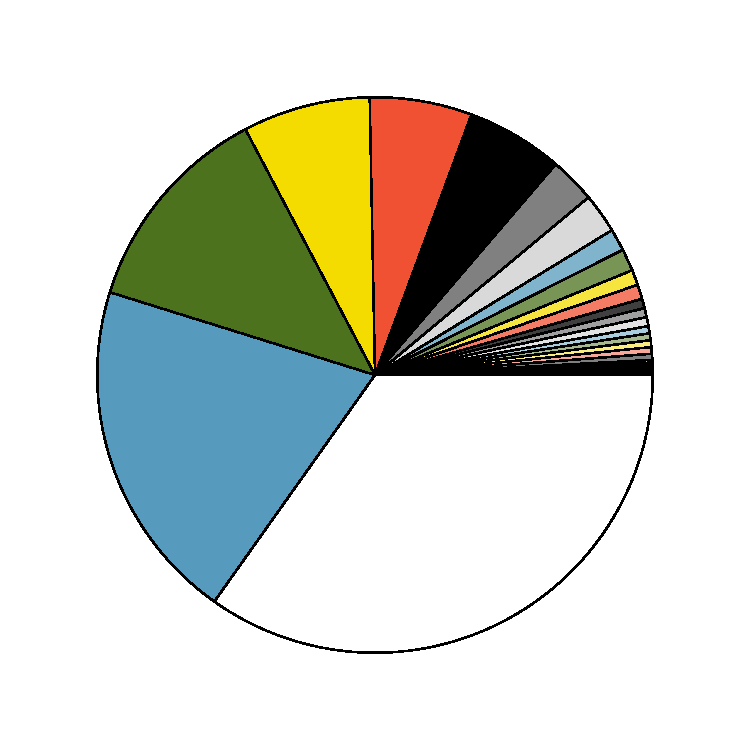
\includegraphics[width=0.4\textwidth]{1-7_categorical_data/figures/mammal_pie_chart/mammal_pie_chart}
%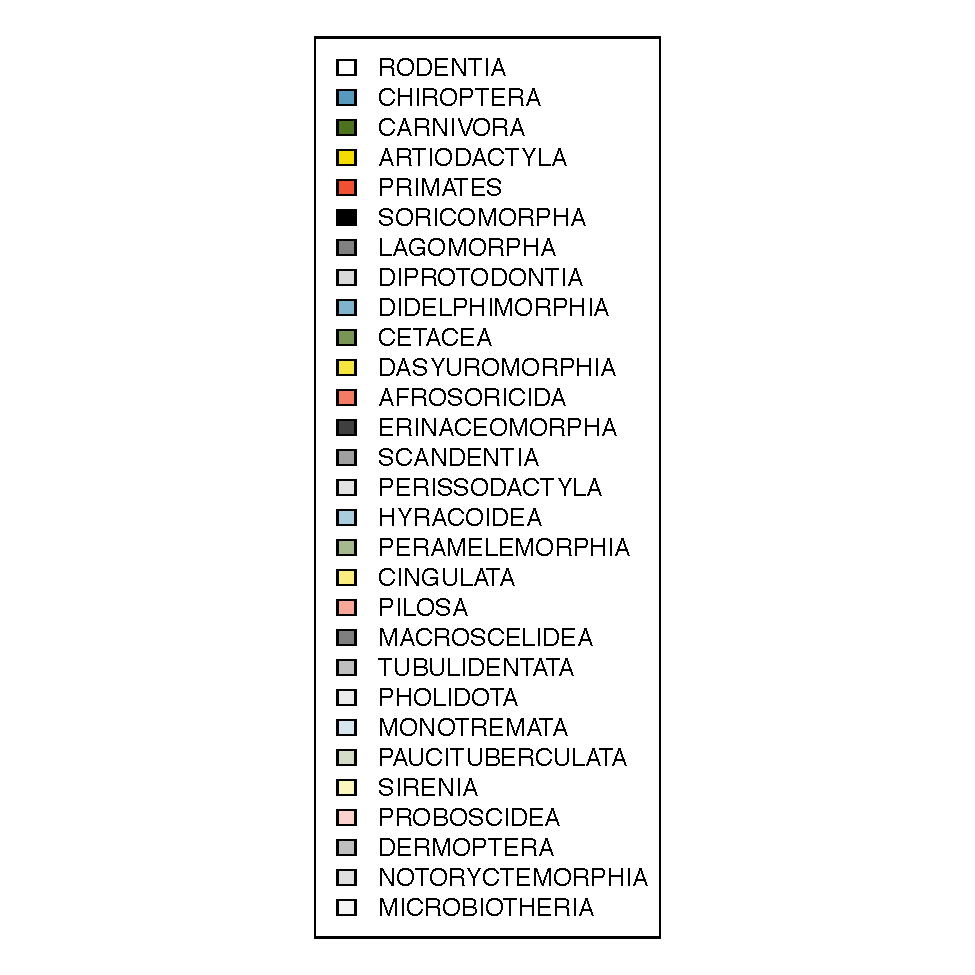
\includegraphics[width=0.2\textwidth]{1-7_categorical_data/figures/mammal_pie_chart/mammal_pie_chart_legend}
%\end{center}

%\ct{Data from \webURL{http://www.bucknell.edu/msw3}.}

%\end{frame}


%%%%%%%%%%%%%%%%%%%%%%%%%%%%%%%%%%%%%

%\subsection{Comparing numerical data across groups}

%%%%%%%%%%%%%%%%%%%%%%%%%%%%%%%%%%%%%

%\begin{frame}
%\frametitle{Side-by-side box plots}

%\dq{Does there appear to be a relationship between class year and number of clubs students are in?}

%\begin{center}
%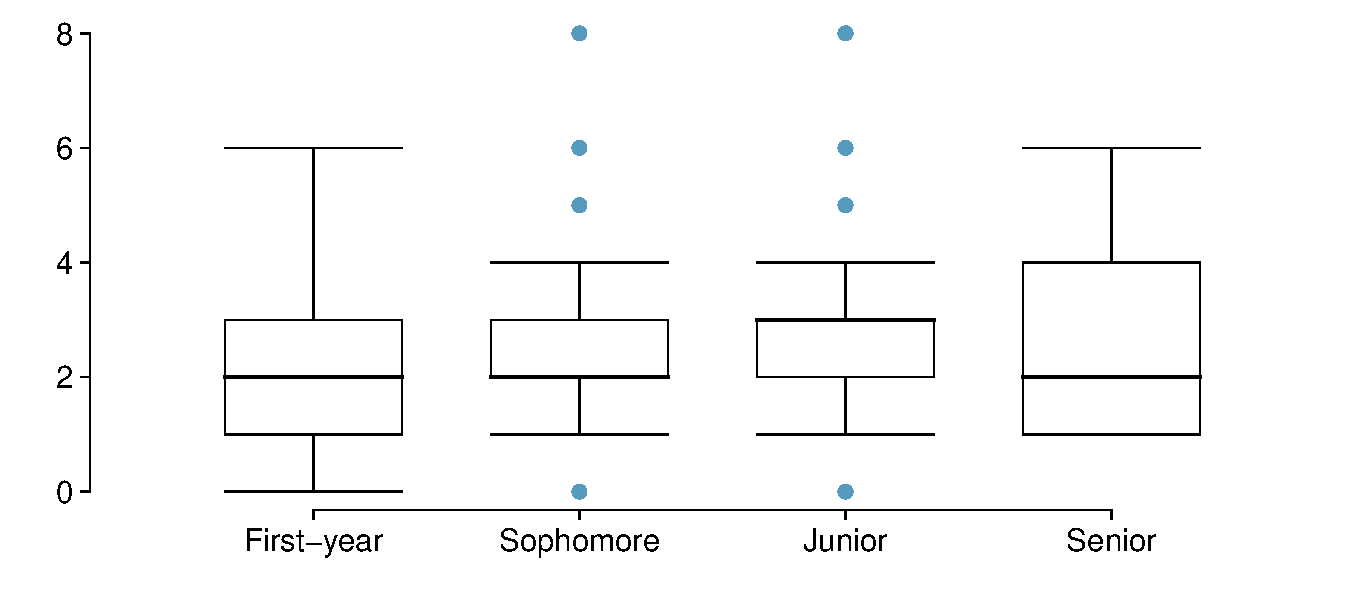
\includegraphics[width=\textwidth]{1-7_categorical_data/figures/year_clubs/year_clubs}
%\end{center}

%\end{frame}

%%%%%%%%%%%%%%%%%%%%%%%%%%%%%%%%%%%%%

